\documentclass[12pt,a4paper]{article}
\usepackage{better_poster}
\graphicspath{{images/}}

% ---- fill in from here

% authors
\title{A Distributed Denial Of Service (DDOS) is an attack in which the perpetrator seeks to make a machine or service unavailable to its intended users.}
\author{Max Sepulveda}

% type of poster: [exp]erimental results, [methods], [theory]
% Disclaimer: the original classification had "study" and "intervention" as separate categories. I group them under experimental results.
\newcommand\postertype{exp} % [exp],[methods],[theory]

\begin{document}

% main point of your study
\makefinding{Increase in volume and number of DDOS between 2018 and 2019}


% \makemain{
% }{

% }
% the main text of your poster goes here
\makemain{
    % you can have 1 or 2 columns
    \raggedcolumns
    \begin{multicols}{2}
    
        \section{DDOS }
        You can also think of it as a person (perpetrator) blocking the entry of a coffee and this prevents other people (intended user) to enter the coffee (website or target)
        
        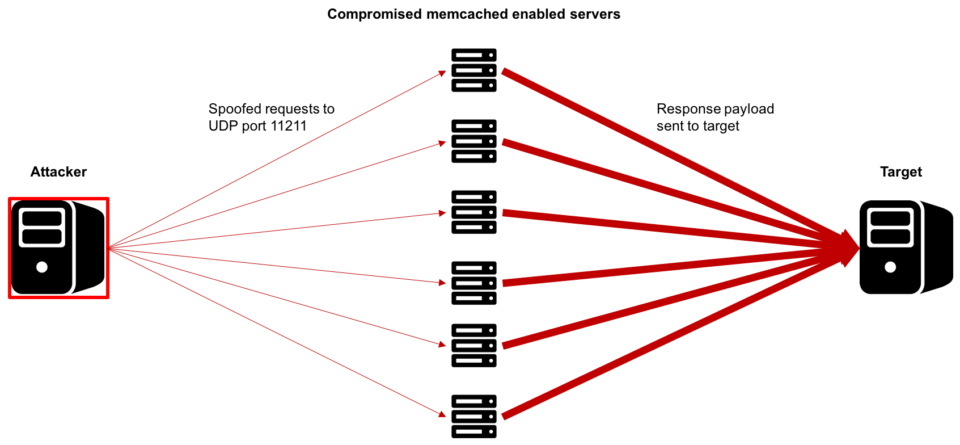
\includegraphics[width=0.85\linewidth]{ddos.png}
            
        \section{Comparison of size}
        $58\%$ of attacks in 2018 were bigger than 5GB/s,  it looks like perpetrators are moving into larger attacks?

        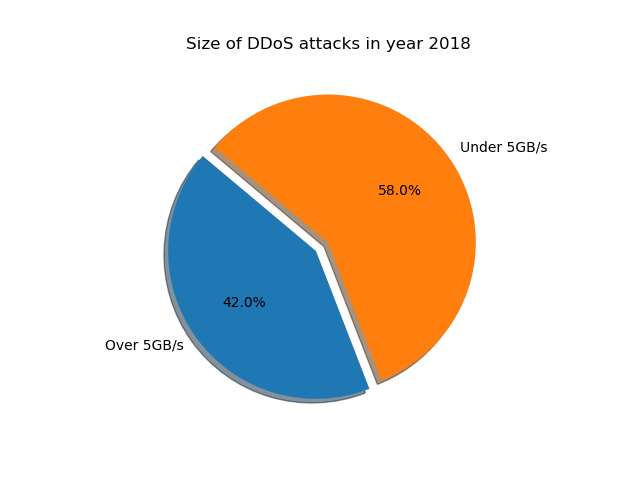
\includegraphics[width=0.85\linewidth]{SizeAttacks.png}
        
    % this determines where your columns will be separated
    \columnbreak

       \section{Volume of the attacks}
       A massive increase on the volume attacks Q1 2018 - Q1 2019.
       
        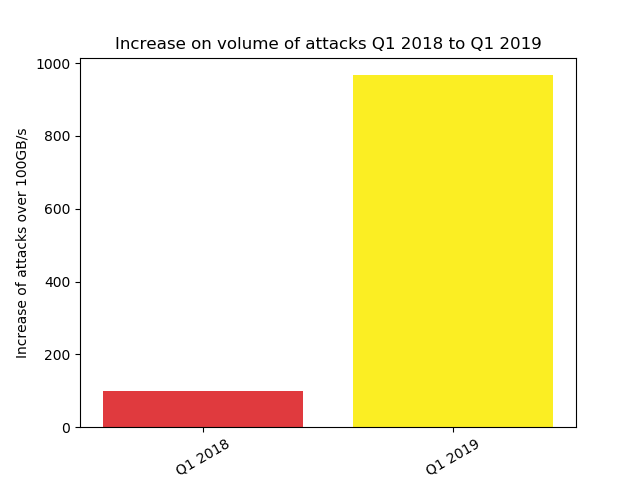
\includegraphics[width=0.8\linewidth]{IncreaseGraph.png}
        
        \section{Number of the attacks}
        Increase on attacks comparing the start of 2018 to the start of 2019.
        
        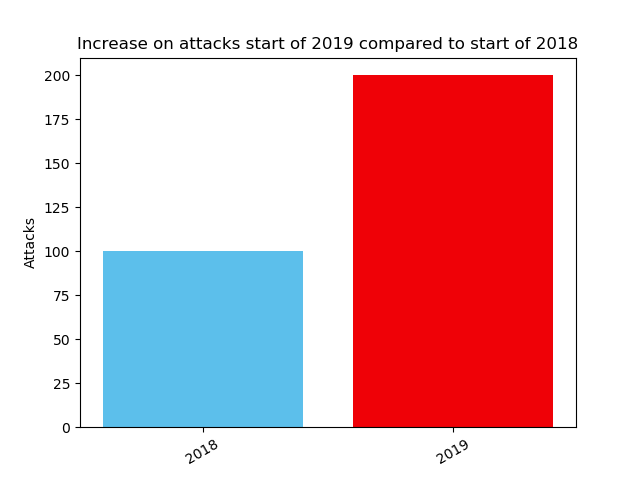
\includegraphics[width=0.8\linewidth]{increase3.png}
    
    \end{multicols}
}

% footer
% generate qr code from https://www.qr-code-generator.com/ and replace qr_code.png
% default: barcode on the left
\makefooter{LVS_Ascot_arms.jpg}{qr-code-rr.png}

% replace with this like for barcode on the right
%\makealtfooter{images/uni_logo.png}{images/qr-code.png}
 
\end{document}